\documentclass{article}

% The geometry package allows for easy page formatting.
\usepackage{geometry}
\geometry{letterpaper}

% Load up special logo commands.
\usepackage{doc}

% Package for formatting URLs.
\usepackage{url}

% Packages and definitions for graphics files.
\usepackage{graphicx}
\usepackage{epstopdf}
\DeclareGraphicsRule{.tif}{png}{.png}{`convert #1 `dirname #1`/`basename #1 .tif`.png}

%
% Set the title, author, and date.
%
\title{Usability of Security Mechanisms in Ubiquitous Computing Environments}
\author{Joaquin Loustau}
\date{October 16, 2014}

%
% The document proper.
%
\begin{document}

% Add the title section.
\maketitle

% Add an abstract.
\abstract{
Describe your paper in 100-200 words, give or take.  The command-line \texttt{wc} utility is really useful here!  This particular sample paper is meant to demonstrate a variety of \LaTeX\ directives for producing a well-structured, consistently-formatted scholarly document.  The actual content and outline may vary according to the needs of your specific research topic.
}

% Add various lists on new pages.
\pagebreak
\tableofcontents

% Start the paper on a new page.
\pagebreak

%
% Body text.
%
\section{Introduction}
\label{introduction}
The International Telecommunication Union, a specialized agency of the United Nations (UN) that is responsible for issues that concern information and communication technologies, reported that mobile phones will outnumber people on Earth by the end of 2014. \cite{} Today, demonstrating the value of ubiquitous computing (ubicomp), the cell phone, or more precisely the “smart phone,” takes center stage crossing a threshold of processor performance, memory capacity and connectivity both cell and local, making it the most widely adopted and ubiquitous computer there has ever been. 

However, the smartphone is just one of several ubiquitous computing devices we encounter during any given day. The future of ubiquitous computing foresees networked microprocessors embedded in everyday objects: not just smart phones and home appliances but furniture, books, sprinklers, etc. ---hundreds of internet-enabled computers communicating to each other over wireless links. 
As the number of ubiquitous computing devices continues to grow, the sheer amount, nature and complexity of the information exchanged will grow exponentially. If the ubicomp systems deployed in our homes, workplaces and vehicles are as vulnerable as today’s personal computers, the implications could be catastrophic. For example, inadequate manipulation of data handled by heart monitors in a clinic or an alarm system for a nuclear power plant could be fatal. The examples are endless. Security is needed to ensure exact and accurate confidentiality, integrity and authentication.

This paper aims to examine the security issues for ubiquitous computing and produce a usability analysis of the log-in and password mechanism of securing information, along with a brief story of previous works and accomplishments in the corresponding areas. 

\section{Background, Preliminary, and Related Work}
The term ubiquitous computing was coined by Mark Weiser, chief technology officer at Xerox’s Palo Alto Research Center (PARC) in 1988 to describe a future in which computers, embedded in everyday objects, replace personal computers (PCs). In his ground-breaking article, ‘The Computer for the 21st Century,” Weiser expresses, “the most profound technologies are those that disappear. They weave themselves into the fabric of everyday life until they are indistinguishable from it.”\cite{}

Presently, ubiquitous computing, or ubicomp, is the term given to the third era of modern computing. The first era was defined by the mainframe computer, a single large-time shared computer owned by an organization and used by several individuals at the same time. Second, came the era of the PC, a personal computer predominantly owned and used by one individual, and dedicated to them. Finally, the third and present era, ubiquitous computing, is characterized of small networked computer products, such as smart phones, tablets, and embedded computers built into many of the devices we own ---resulting in a world in which each person uses hundreds of computers a day.

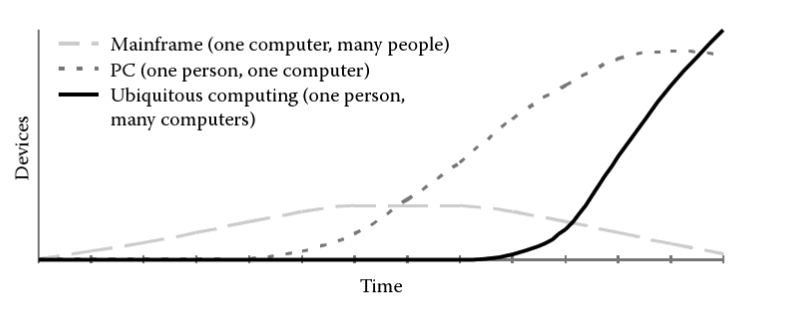
\includegraphics[scale=.6]{eras_modern_computing.png}

Rich Gold, a member of Dr. Weiser’s team at PARC, proposed a taxonomy of properties for ubiquitous computing based on Weiser’s formulations. The properties were: sensuous, reactive, communicative, embedded socially and colonizing. 

In addition to ubiquitous computing, the other major topic that this paper will cover is security. Amoroso defines computer security as risk management: assessing threats, vulnerabilities and attacks, estimating costs for the threats, estimating probabilities for the attacks given the vulnerabilities, developing appropriate safeguards (a priori vaccines) and countermeasures (a posteriori remedies), and implementing the ones for which the certain price of the defense is worth spending compared to the uncertain loss that a potential threat implies. 

The required characteristics of a secure system are often summarized in the acronym CIA. This does not refer to Central Intelligence Agency but is instead a widely used benchmark for evaluation of information systems security, focusing on the three core goals of confidentiality, integrity and availability of information. Confidentiality refers to limiting information access and disclosure to authorized users. Integrity is the property that refers to the trustworthiness of information resources and is violated whenever information is altered in an unauthorized way. Finally, availability is the property of a system which always ensures that information is accessible when needed. 

The efforts to mitigate the risks of threats to confidentiality, integrity and availability often take the form of user authentication. User authentication is a basic theme in computer security and covers establishing who the user is (identification), verifying this identity (verification or authentication), and providing proper access to the resource that the user is allowed to use (authorization). 

Finally, this paper will analyze the usability of a specific authentication mechanism, the traditional login schema. It would therefore be desirable to define the term usability in this context. The ISO 9241-11 Guidance on Usability from the year 1998, issued by the International Organization for Standardization, defines usability as: “The extent to which a product can be used by specified users to achieve specified goals with effectiveness, efficiency and satisfaction in a specified context of use.”

\section{Methods}
In order to investigate the topic of Usability of Security Mechanism in Ubiquitous Computing Environments, a top-down approach was employed. Firstly, one performed an exhaustive search of articles, books and journals covering Usability, Security and Ubiquitous Computing as independent concepts. The two main sources chosen for this search were the William H. Hannon Library at Loyola Marymount University and the Association for Computing Machinery’s (ACM) Digital Library.  

A narrower and more specific search for materials was then conducted, and sources cited in the selected articles were explored, thus unveiling a myriad of different publications. To assess the reliability of these new sources, Google Scholar was a significantly important tool. Google Scholar provides information such the number of times the given article has been cited as well as the sources of these citations.  Articles that have been cited time and again and have been published or cited by prestigious scientific journals are most likely to be reliable.

Organizations such as the Association for Computing Machinery (ACM) or the Institute of Electrical and Electronics Engineers (IEEE) are known for their academic rigor, and consequently provide an almost certain guaranty of the credibility and authority of the pieces appearing in their publications. 


\section{Discussion}
While there is extensive bibliography on different strategies to secure information systems , the significantly smaller number of sources available on usability of security mechanisms sheds lights on the fact that the design and usability of user authentication mechanisms is an often overlooked feature of computer systems.
As people become more connected electronically, the ability to achieve a highly accurate and user-friendly automatic personal identification system is substantially more critical. \cite{jain} The usability of security of security mechanisms is not just a question of improving interfaces to security tools, but designing security to work with the real-world task users perform, and within the physical and social context of that interaction. 
The most common and widespread security mechanism is the login-password schema. This approach is most suitable for office situations, where individuals work on a single personal computer for a long period of time ---generally a whole working day. The usability of using a login and password for every ubicomp device does not seem to be clear. 

The number of devices a user will interact with will require multiple usernames and passwords for the user to remember. Remembering usernames and passwords is difficult even for experienced computer users and typing them in, created a breakdown in the interaction with the computer, forcing the user to focus on the device rather than on his or her task at hand.  De Alvare \cite{} discovered that once a password is chosen, a user is unlikely to change it until it has been compromised. Furthermore, users also tend to construct passwords that contain the least amount of characters as possible.

Similarly, mechanisms and policies for increasing the password strength like frequent change of passwords or requesting a password of a certain length that includes different kinds of symbols, often has the opposite effect as users make easy-to-remember passwords and write them down, thereby lowering security. This shows how a highly secure system from a technical standpoint can be made insecure if the authentication is difficult or tedious to use. The result is that users find ways to circumvent and shortcut the security system, which leads to vulnerable systems. 
The two alternatives to the log-in/password method often suggested are tokens and biometrics. A security token (also sometimes called authentication token) is a small hardware device that the owner carries to authorize access to a network service. The device may be in the form of a smart card or may be embedded in a commonly used object such as a key fob. 

Security tokens may provide an extra level of assurance through a method known as two factor authentication: the user has a personal identification number (PIN), which authorizes them as the owner of that particular device; the device then displays a number which uniquely identifies the user to the service, allowing them to log in. However, as a physical token, smartcards or other forms of security tokens are subject to be lost or stolen.  

Biometric identifiers exploit certain physiological or behavioral characteristics that are distinctive to each person, and thus are more reliable and more capable than knowledge-based and token-based techniques in differentiating between authorized and unauthorized users. By using biometrics system people can be identified by something they are instead of something they have (e.g., a smart card) or know (e.g., their password and login).
An ideal biometric should be universal, where each person possess the characteristics, unique, where no two people should share the characteristic; permanent, where the characteristic should neither change nor be alterable; and collectable, where the characteristic is readily presentable to a sensor and is easily quantifiable. In practice, however, a characteristic that satisfies all these requirements may not always be feasible for a useful biometric system. \cite{}
There are eight biometric types that are currently being used in systems: face geometry, fingerprint, hand geometry, iris pattern, retinal pattern, signature, voice print, and facial thermogram. Even though it is being ‘marketed’ as a new user-friendly user authentication mechanism, there is little research so far into the usability of these systems. Most work and research on biometric systems focus on security and accuracy. 
A traditional way of testing a biometric system is to measure the correlation between the false-acceptance rate (FAR) ---the percentage of unauthorized users incorrectly matched to a valid user’s biometric--- and the false-rejection rate (FRR) ---the percentage of incorrectly rejected valid users. Biometric specialists normally agree that the biometric rates of FAR and FRR are the equivalent of the password space in PIN/Password based authentication.\cite{} Biometrics do not provide perfect (unique) identification. The matching process is probabilistic and is subject to statistical error.    The UK Government Biometrics Working Group (BWG) expressed in their “Biometric Security Concerns” that current knowledge of biometric algorithm behavior and human feature randomness and variation does not permit theoretical analysis of biometric system performance. \cite{}

The key to finding an appropriate security mechanism for an ubicomp environment should consequently not focus so much on the technical aspect but should instead have usability as a primary motivation or goal.  Zurko and Simon \cite{} refer to this approach as user-centered security, and one subscribes to this concept. 

As it has already been mentioned, the traditional login schema completely disrupts a smooth flow of work in the settings prescribed by a ubiquitous computing environment. As users abandon a static room with its desktop computer for a world in which every device offers computer support, the aspects of mobility, cooperation, interruption, and sharing of material become core aspects of much real world work. The design of security systems for this kind of working environments needs to accommodate such challenges, rather than unconsciously adopt existing user authentication mechanisms.
The first security application to articulate a user-centered design philosophy was Privacy-Enhanced Mail (PEM).\cite{linn} "The set of supported measures offers added value to users, enhancing rather than restricting the set of capabilities available to users." This was a startling vision in the security community that largely perceived security requirements as watching and restricting users. While usability problems with the certificate authority infrastructure kept PEM from being widely deployed, its primary motivation to offer users desirable security services such as privacy for their daily electronic mail remains a laudable goal still  unmet today.  This example shows that considerations for users' natural working patterns can strengthen the security of the system. (User-Centered Security, Zurko-Simon)
 
While the implementation details of a suitable security mechanism for an ubicomp environment may vary, one believes they should accomplish the following five objectives:

\begin{enumerate}
 \item \textbf{Allow for proximity-based user authentication.}
 \item \textbf{Support migrating user session within devices.}
 \item \textbf{Easy transition between users in the same device/allow mult-iuser sessions.}  
 \item \textbf{Flexibility to create and/or delete new users (for users authorized to do so).}
 \item \textbf{Common procedures and interfaces within devices when deemed possible.}
\end{enumerate}

\section{Conclusions}
As user-interface technology continues to evolve and users' needs continue to diversify at an unprecedented pace, no single technology or architecture is always ``user friendly.” 

The paradigm should be the full integration of security and usability concerns into the software development process, thus enabling developers to build secure systems that work in the real world. \cite{flechais}

\bibliography{assignment1016}
\bibliographystyle{plain}

\end{document}
